\section{Numerical Simulations}
\begin{comment}
\begin{frame}{Accuracy Study}
	\scriptsize
	The scheme can be specified by three integers $(m_1, m_2, m_3)$, which represent the following [LeVeque et. al]:
	\begin{align*}
		m_1 &= \left\{
		\begin{array}{ll}
			1, & \parbox[t]{0.6\textwidth}{The second order correction wave is not included,\\
				thus the method is formally first order accurate.} \\
			0, & \text{The correction wave is included.}
		\end{array}
		\right. \\
		m_2 &= \left\{
		\begin{array}{lll}
			0, & \text{No transverse propagation.} \\
			1, & \text{The propagation of the increment wave.} \\
			2, & \text{Transverse propagation of both increment and correction wave.}
		\end{array}
		\right. \\
		m_3 &= \left\{
		\begin{array}{lll}
			0, & \text{No double transverse propagation.} \\
			1, & \text{Double transverse propagation of the increment wave.} \\
			2, &  \parbox[t]{0.6\textwidth}{Double transverse propagation of both increment and \\
				correction wave.}
		\end{array}
		\right.
	\end{align*}
\end{frame}
\end{comment}

\begin{frame}{Coupled System for a Three-Dimensional Flow}
	\scriptsize
	We consider $\boldsymbol{u} = \left( 0, 0, w(x,y,z,t)\right)^T$, $f(x,y,t,\phi,\theta)$. We get
	\begin{equation}
		\begin{aligned}
			&\sin\theta \partial_{t}f(x,y,t,\phi, \theta)+ \textcolor{red}{\partial_x(\cos\phi \sin\theta \cos\theta f)} + \textcolor{red}{\partial_y(\sin \phi \sin \theta \cos \theta f)} - \textcolor{red}{\partial_z((1+ \cos^2 \theta)f)} \\
			&= -  \textcolor{blue}{\partial_\theta\left(( w_x \sin^3 \theta \cos \phi + w_y\sin \phi \sin^3 \theta - w_z \cos \theta \sin^2 \theta) f\right)} \textcolor{blue}{D_{r}\left( \partial_\phi \left(\frac{1}{\sin \theta} \partial_\phi f \right)+ \partial_\theta (\sin \theta \partial_\theta f)\right)} \\
			&Re\partial_{t}w(x,y,t) = \partial_{xx}w + \partial_{yy}w + \partial_{yy}z + \delta\left(\bar{\rho}-\int_{0}^{2\pi} \int_{0}^{\pi} f \sin \theta d\theta d\phi \right).
		\end{aligned}
	\end{equation}
	\pause
	The system of hierarchy of moment equations is given as
	\begin{equation}
		\partial_t Q + \textcolor{red}{A  \partial_x Q}
		+ \textcolor{red}{B \partial_y Q} +  \textcolor{red}{C \partial_z Q} =  \textcolor{blue}{ D(w_x,w_y, w_z)Q+ D_rEQ},
	\end{equation}
	where $Q=(c^0_0(x,t), c^{-2}_2(x,t), \ldots, c^{2N}_{2N}(x,t))^T$ represents the vector of the moments and \\
	\vspace{2mm}
	$A,B,C,D,E \in \mathbb{R}^{(N+1)(2N+1)x(N+1)(2N+1)}$.
\end{frame}

\begin{frame}{Wave Propagation and Error Analysis}
	\scriptsize
	\textbf{Wave propagation parameters (LeVeque et al.):}
    The scheme can be characterized by three integers $(m_1, m_2, m_3)$:
	\begin{itemize}
		\item $m_1$: Correction wave (1 = not included, 2 = included)
		\item $m_2$: Transverse propagation (0 = none, 1 = increment only, 2 = increment + correction)
		\item $m_3$: Double-transverse propagation (0 = none, 1 = increment only, 2 = increment + correction)
	\end{itemize}
	
	\medskip
	\textbf{Error computation:}  
	On a coarse grid, define
	\[
	E(h) = U(h) - U(h/2), \quad
	E(h/2) = U(h/2) - U(h/4)
	\]
\end{frame}

%-------------------------------------------------------

\begin{frame}{Accuracy Analysis}
	\scriptsize
	
	% Initialwert direkt über der Tabelle
	Let 
	\[
	r = \sqrt{(x-40)^2+(y-30)^2+(z-50)^2}, \quad
	c^0_0(x, y, k, 0) = \exp(-0.01 \, r^2)
	\] 
	be the initial value.
	
	\medskip
	\centering
	\begin{tabular}{|c|c|c|c|c|c|c|c|}
		\hline
		Method & Grid & \multicolumn{2}{c|}{N=1} & \multicolumn{2}{c|}{N=2} & \multicolumn{2}{c|}{N=7} \\
		\cline{3-8}
		&  & $L_1$ Error & EOC & $L_1$ Error & EOC & $L_1$ Error & EOC \\
		\hline
		(1,1,1) & 32  & $5.57\cdot10^{-4}$ & -    & $5.47\cdot10^{-4}$ & -    & $5.01 \cdot10^{-4} $ & - \\
		& 64  & $3.54\cdot10^{-4}$ & 0.65 & $3.40\cdot10^{-4}$ & 0.68 & $2.93\cdot10^{-4}$ & $0.77$ \\
		& 128 & $1.79\cdot10^{-4}$ & 0.98 & $1.80\cdot10^{-4}$ & 0.91 & - & - \\
		\hline
		(2,2,2) & 32  & $1.79\cdot10^{-4}$ & -    & $2.00\cdot10^{-4}$ & -    & $1.83\cdot10^{-4}$ & - \\
		& 64  & $4.66\cdot10^{-5}$ & 1.94 & $5.45\cdot10^{-5}$ & 1.86 & $4.82\cdot10^{-5}$ & 1.92 \\
		& 128 & $1.17\cdot10^{-5}$ & 1.99 & $1.38\cdot10^{-5}$ & 1.98 & - & - \\
		\hline
	\end{tabular}
	
	\vspace{0.5em}
    \footnotesize{
	\textbf{Table:} Accuracy analysis for the component $c^0_0$ of the coupled 3D flow problem ($D_r=1$). The time step was limited by the CFL condition, with $cfl \le 0.45$ for method (1,1,1) and $cfl \le 0.9$ for method (2,2,2).  
}
\end{frame}

%-------------------------------------------------------


\begin{frame}
	\scriptsize
		\begin{figure}[H]
			\centering
			\begin{minipage}{0.4\textwidth}
				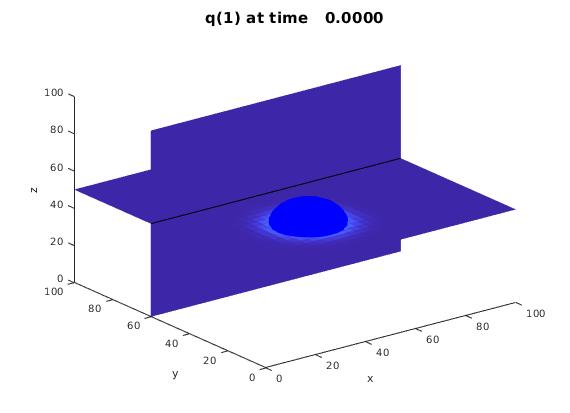
\includegraphics[scale=0.26]{Bilder_3D/Example_1Glocke_t=0_T22}
			\end{minipage}
			\hfill 
			\begin{minipage}{0.4\textwidth}
				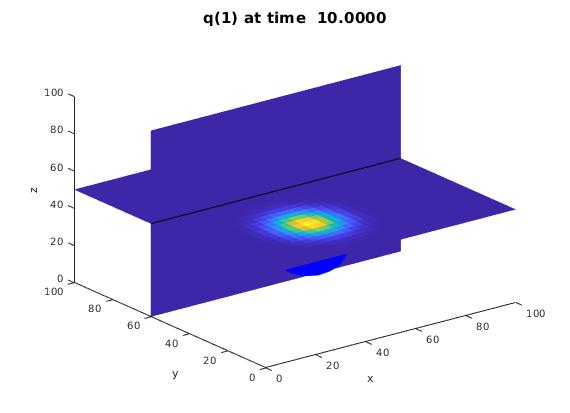
\includegraphics[scale=0.26]{Bilder_3D/Example_1Glocke_t=10_T22}
			\end{minipage}
		\end{figure}
		\begin{figure}[H]
			\centering
			\begin{minipage}{0.4\textwidth}
				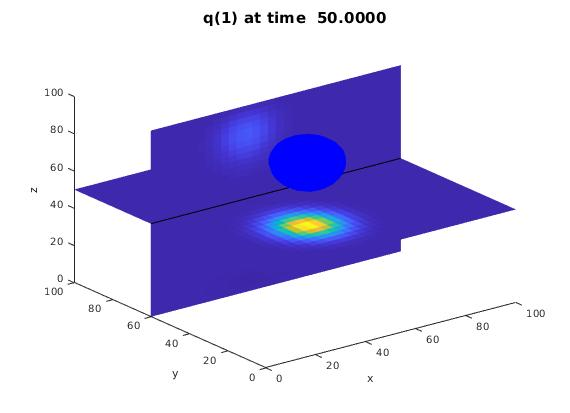
\includegraphics[scale=0.26]{Bilder_3D/Example_1Glocke_t=50_T22}
			\end{minipage}
			\caption{Numerical results for $c^0_0$ at different times using $D_r=1$, $w_x=w_y=1$ and $w_z=0$.}
		\end{figure}
\end{frame}
